\documentclass[11pt,a4paper]{paper}

\usepackage[T1]{fontenc}

\usepackage{graphicx}
\usepackage{amssymb}
\usepackage{amstext}
\usepackage{amsmath}
\usepackage{a4wide,color}
\usepackage[utf8]{inputenc}
\usepackage[frenchb]{babel}
\usepackage{xspace}
\usepackage{anysize}
\usepackage{tabularx}
\usepackage{multirow}
\usepackage{fancybox}
\usepackage{fancyhdr}
\usepackage{bbding}

\usepackage{multicol}

\setlength{\parskip}{1ex plus 0.5ex minus 0.2ex}
\usepackage{color}
\usepackage{float}

\usepackage[toc,page]{appendix} 
\usepackage{lscape}

\usepackage{placeins}

\usepackage{listingsutf8}
%\usepackage{listings}

\usepackage{todonotes}

\lstset{% general command to set parameter(s)
	basicstyle=\footnotesize, % print whole listing small
	keywordstyle=\color{magenta}\bfseries, % underlined bold black keywords
	identifierstyle=, % nothing happens
	commentstyle=\color{black}, % white comments
	stringstyle=\ttfamily, % typewriter type for strings
	showstringspaces=false % no special string spaces
} 

\lstdefinelanguage{aald}
	{morekeywords={system, implementation},
	sensitive=false,
	morecomment=[l]{//},
	morecomment=[s]{/*}{*/},
	morestring=[b]",
}

\usepackage[colorlinks=true]{hyperref}

\renewcommand{\appendixtocname}{Annexes} 
\renewcommand{\appendixpagename}{Annexes}

\usepackage[normalem]{ulem}
\usepackage{color}

\definecolor{Fond}{gray}{0.7}

\renewcommand{\floatpagefraction}{.99}
\renewcommand{\textfraction}{.01}
\newcommand{\modif}[1]{\textcolor{red}{\uline{#1}}}


\pagestyle{fancy}
\fancyhf{}
\fancyhead[RE,RO]{\thepage}
\fancyhead[LE]{}
\fancyhead[LO]{Programmation et conception de systèmes temps réel -- 4ème année AE et IR}
\fancyfoot[LO]{INSA Toulouse -- \today}
\fancypagestyle{plain}{%
  \fancyhf{} % get rid of headers
  \renewcommand{\headrulewidth}{0pt} % and the line
}

\newenvironment{maliste}%
{ \begin{list}%
	{\ArrowBoldRightStrobe}%
	{\setlength{\labelwidth}{30pt}%
	 \setlength{\leftmargin}{35pt}%
	 \setlength{\itemsep}{\parsep}}}%
{ \end{list} }




\title{{\Huge Projet De Stijl 2.0}
{\small : Plateforme pour robots mobiles}\\
{\scriptsize Programmation et conception de systémes temps réel -- 4éme année AE/IR}\\
{\scriptsize Institut National des Sciences Appliquées de Toulouse}\\
---\\
Dossier de conception \\
{\large Version 2.0.$\beta$ (\today)}\\
{\scriptsize Référent pédagogique : P.-E. Hladik (\texttt{pehladik@insa-toulouse.fr})}\\
---
}


\begin{document}

\maketitle

%\begin{table}[htdp]
%\caption{Suivi des modifications}
%\begin{center}
%\begin{tabular}{|c|c|c|p{8cm}|}
%\hline
%Date & Version & Auteur & Modifications\\
%\hline
%JJ/MM/12 & 0.3.X & P.-E. Hladik&  \\
%\hline
%\end{tabular}
%\end{center}
%\label{default}
%\end{table}%
%\newpage

%\tableofcontents

%\newpage

%%%%%%%%%%%%%%%%%%%%%%%%%
  \section{Introduction}
%%%%%%%%%%%%%%%%%%%%%%%%%
\label{sec:premier}

Ce document a pour but de vous apprendre à lire un modèle en AADL et les diagrammes d'activité qui décrivent le comportement des threads. Le document présente le résultat d'une conception réalisée à la va-vite. Cette conception ne prend en considération que la mise en place des communications et la gestion des déplacements du robot ce qui correspond aux fonctionnalités 1, 2, 3, 4, 7, 10 et 12 du cahier des charges fonctionnel.

Le code initial qui vous est fourni à la première séance de travaux pratiques correspond à l'implémentation de la conception présentée ici.

Attention, les choix qui ont été faits ne sont pas forcément les meilleurs. Tout ce qui est proposé peut être remis en cause dans la suite du travail. \`A vous d'ajouter, de modifier, de critiquer de manière pertinente cette conception.

%%%%%%%%%%%%%%%%%%%%%%%%%
\section{Diagramme de contexte}
%%%%%%%%%%%%%%%%%%%%%%%%%

La figure~\ref{fig:contexte} présente le superviseur dans son contexte et ses interactions avec les autres composants de la plate-forme.

 \begin{figure}[htbp]
\begin{center}
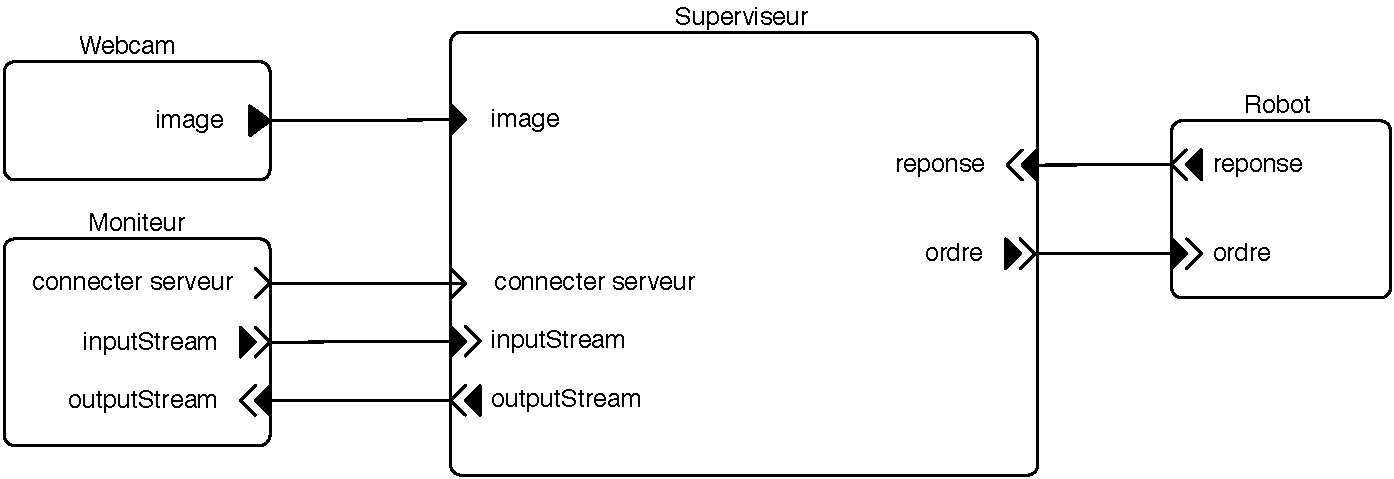
\includegraphics[scale=0.6]{figures_pdf/contexte}
\caption{Diagramme de contexte}
\label{fig:contexte}
\end{center}
\end{figure}
\FloatBarrier

La webcam produit des données (\texttt{image}) sous la forme d'un tableau d'octets. Le robot reçoit des ordres (\texttt{ordre}) sous la forme d'une chaîne de caractères et retourne une réponse aussi sous la forme d'une chaîne (\texttt{reponse}). Le moniteur envoi un événement (\texttt{connecter serveur}) pour demander la connexion avec le serveur puis établit une communication bi-directionnelle sous la forme d'une flux d'octets (\texttt{inputStream} et \texttt{outputStream}).

%%%%%%%%%%%%%%%%%%%%%%%%%
\section{Le travail d'un concepteur : l'analyse fonctionnelle}
%%%%%%%%%%%%%%%%%%%%%%%%%

À partir du cahier des charges, le concepteur va analyser chaque fonctionnalité en se demandant quelles sont les données consommées et produites ainsi que les traitement à réaliser. Petit à petit il va ainsi construire l'architecture du programme.

Dans la suite de ce document, nous ne nous intéresserons qu'aux fonctionnalités 1, 2, 3, 4, 7, 10 et 12 présentées dans le cahier des charges fonctionnel. Votre travail consistera à compléter la conception déjà réalisée pour intégrer l'ensemble des fonctionnalités. Vous pouvez modifier tout ce que vous voulez de cette conception.

En analysant la fonctionnalité 1, le concepteur produit au brouillon le dessin suivant. Il décrit dans un rectangle blanc la fonction et dans une note sur fond jaune le comportement de la fonction. La flèche en pointillée représente un évènement. 
 \begin{figure}[htbp]
\begin{center}
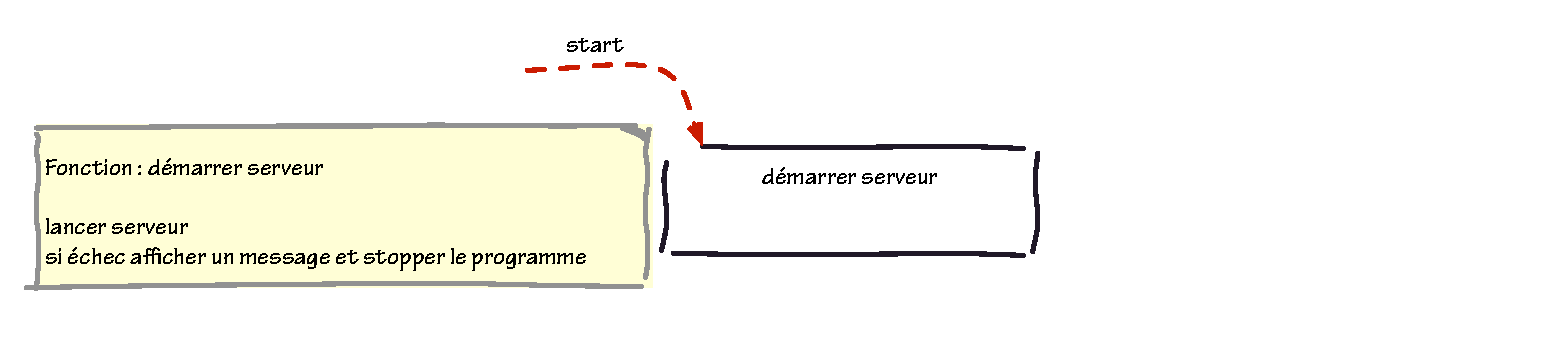
\includegraphics[scale=0.5]{figures_pdf/fonc/fonc1}
\end{center}
\end{figure}
\FloatBarrier

Pour intégrer la fonctionnalité 2, le concepteur complète son brouillon avec une nouvelle fonction. Il modifie aussi la première fonction pour que celle-ci produise l'événement {\tt serveur démarré}. L'évènement {\tt ouvrir socket} est produit par le moniteur lorsque l'utilisateur demande la connexion entre le moniteur et le superviseur.
 \begin{figure}[htbp]
\begin{center}
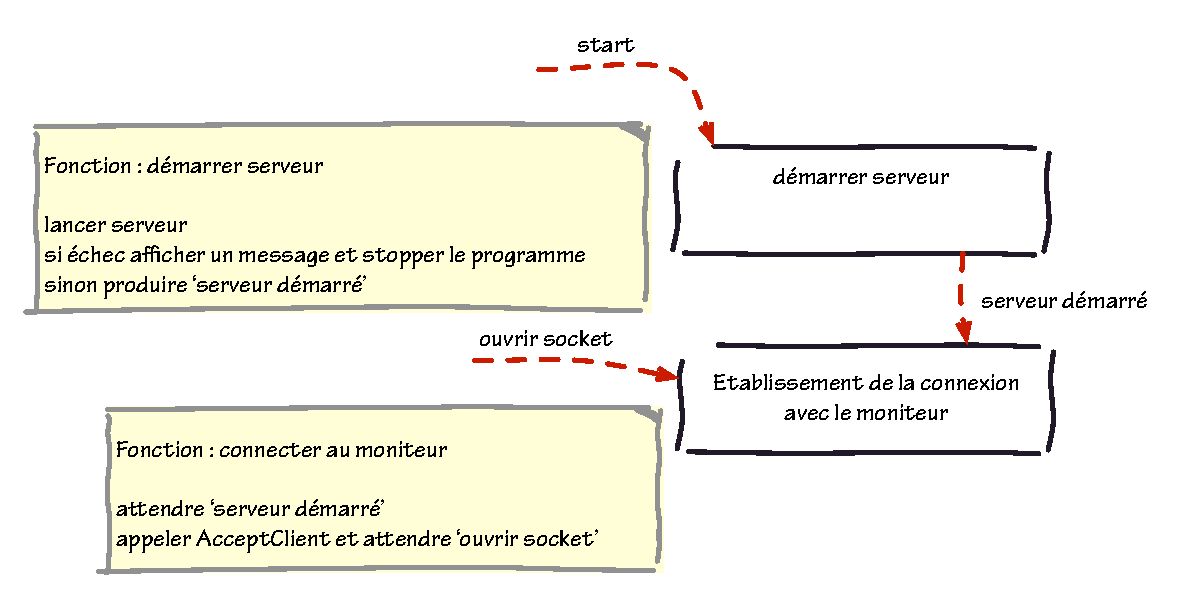
\includegraphics[scale=0.5]{figures_pdf/fonc/fonc2}
\end{center}
\end{figure}
\FloatBarrier

Les fonctionnalités 3 et 4 (voir dessin ci-dessous) induisent l'ajout du nouvel évènement {\tt connexion établie}. Une file de messages {\tt messageToMon} est aussi introduite. C'est dans cette file que seront postés les messages à envoyer au moniteur. On remarque l'apparition des flux de données-événement {\tt inputStream} et {\tt oututStream} en provenance et à destination du moniteur.
 \begin{figure}[htbp]
\begin{center}
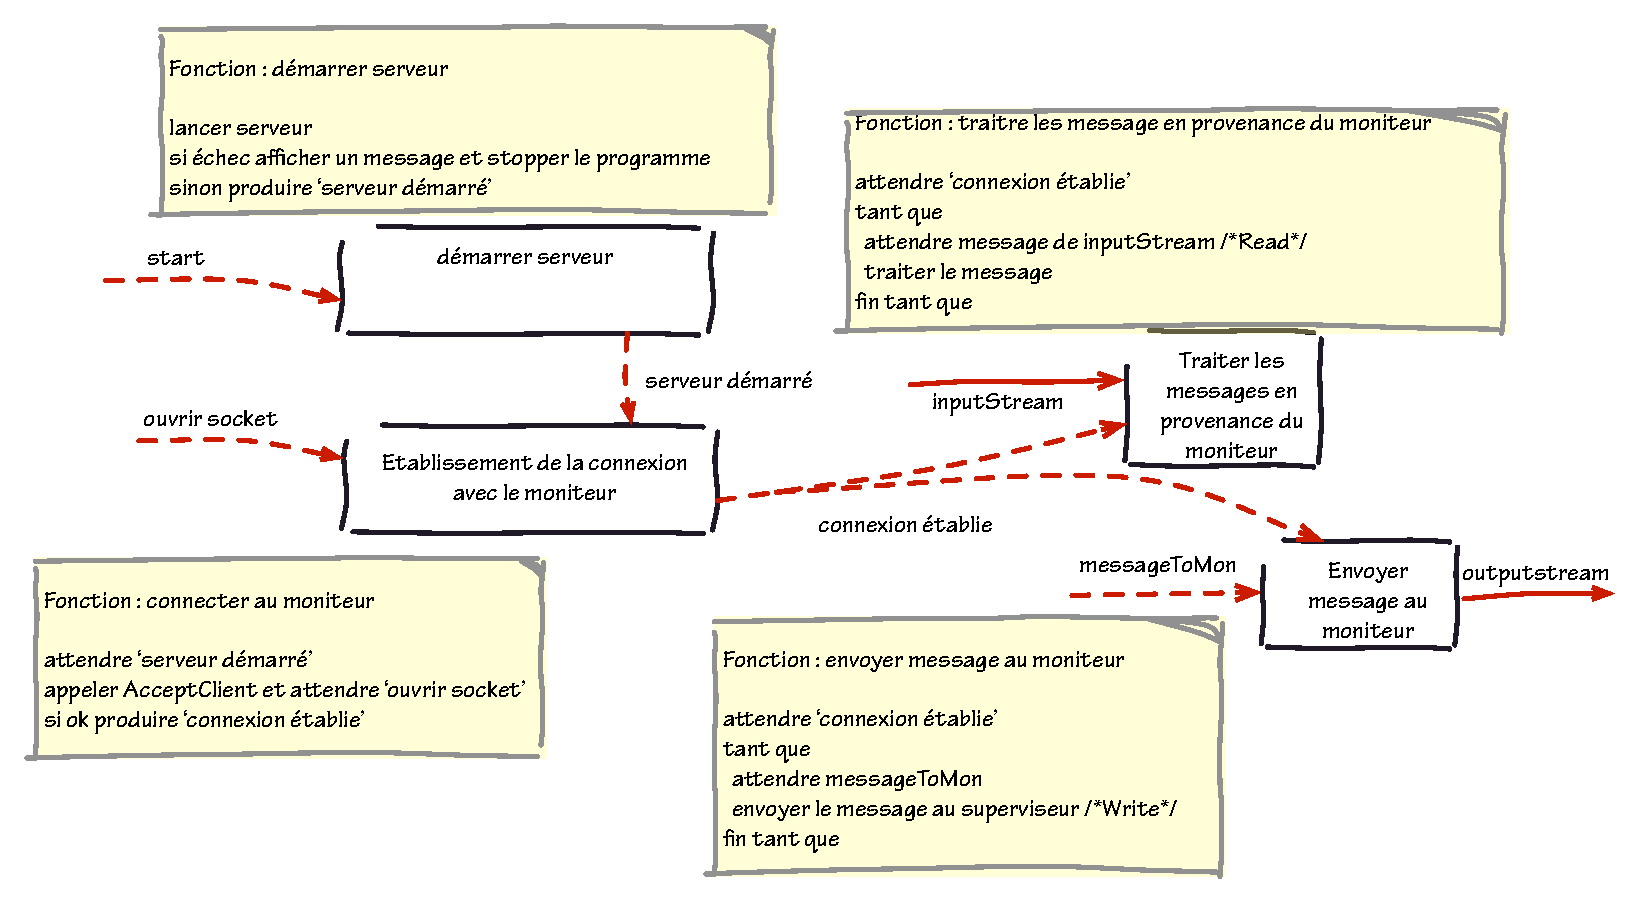
\includegraphics[scale=0.5]{figures_pdf/fonc/fonc3-4}
\end{center}
\end{figure}
\FloatBarrier


L'ajout de la fonctionnalité 7 conduit à modifier la fonction de réception pour différencier les actions à réaliser en fonction du type des messages reçus. Un nouvel évènement {\tt ouvrir comRobot} est ainsi ajouté pour signaler une demander de mise en service de la communication avec le robot. On remarque aussi que la file de messages {\tt messageToMon} est maintenant utilisée par une fonction pour envoyer au moniteur le message d'acquittement ou d'échec.
 \begin{figure}[htbp]
\begin{center}
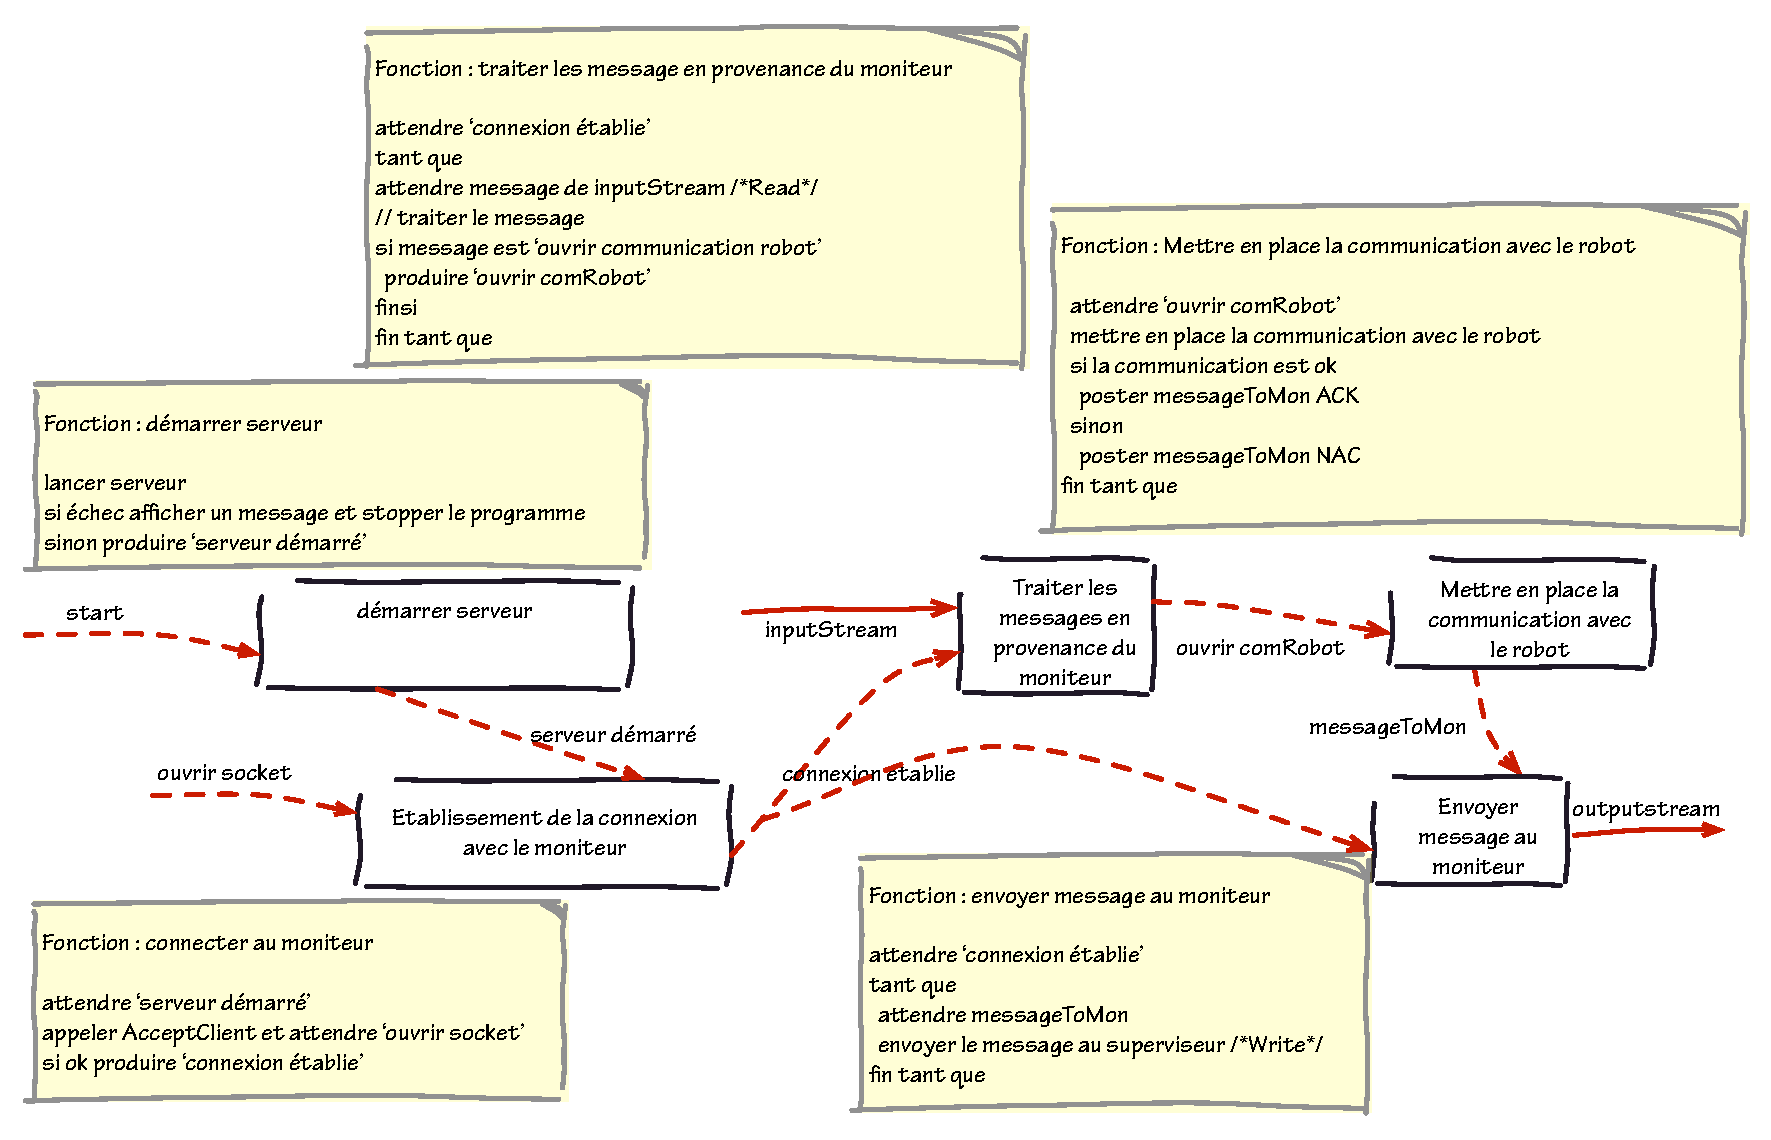
\includegraphics[scale=0.5]{figures_pdf/fonc/fonc7}
\end{center}
\end{figure}
\FloatBarrier

La fonction pour démarrer le robot sans watchdog (fonctionnalité 10) suit le même schéma que le fonctionnalité 7. On remarque cette fois que les flux {\tt ordre} et de {\tt réponse} sont utilisés pour communiquer avec le robot. La file de message {\tt messageToMon} a maintenant deux producteurs.
 \begin{figure}[htbp]
\begin{center}
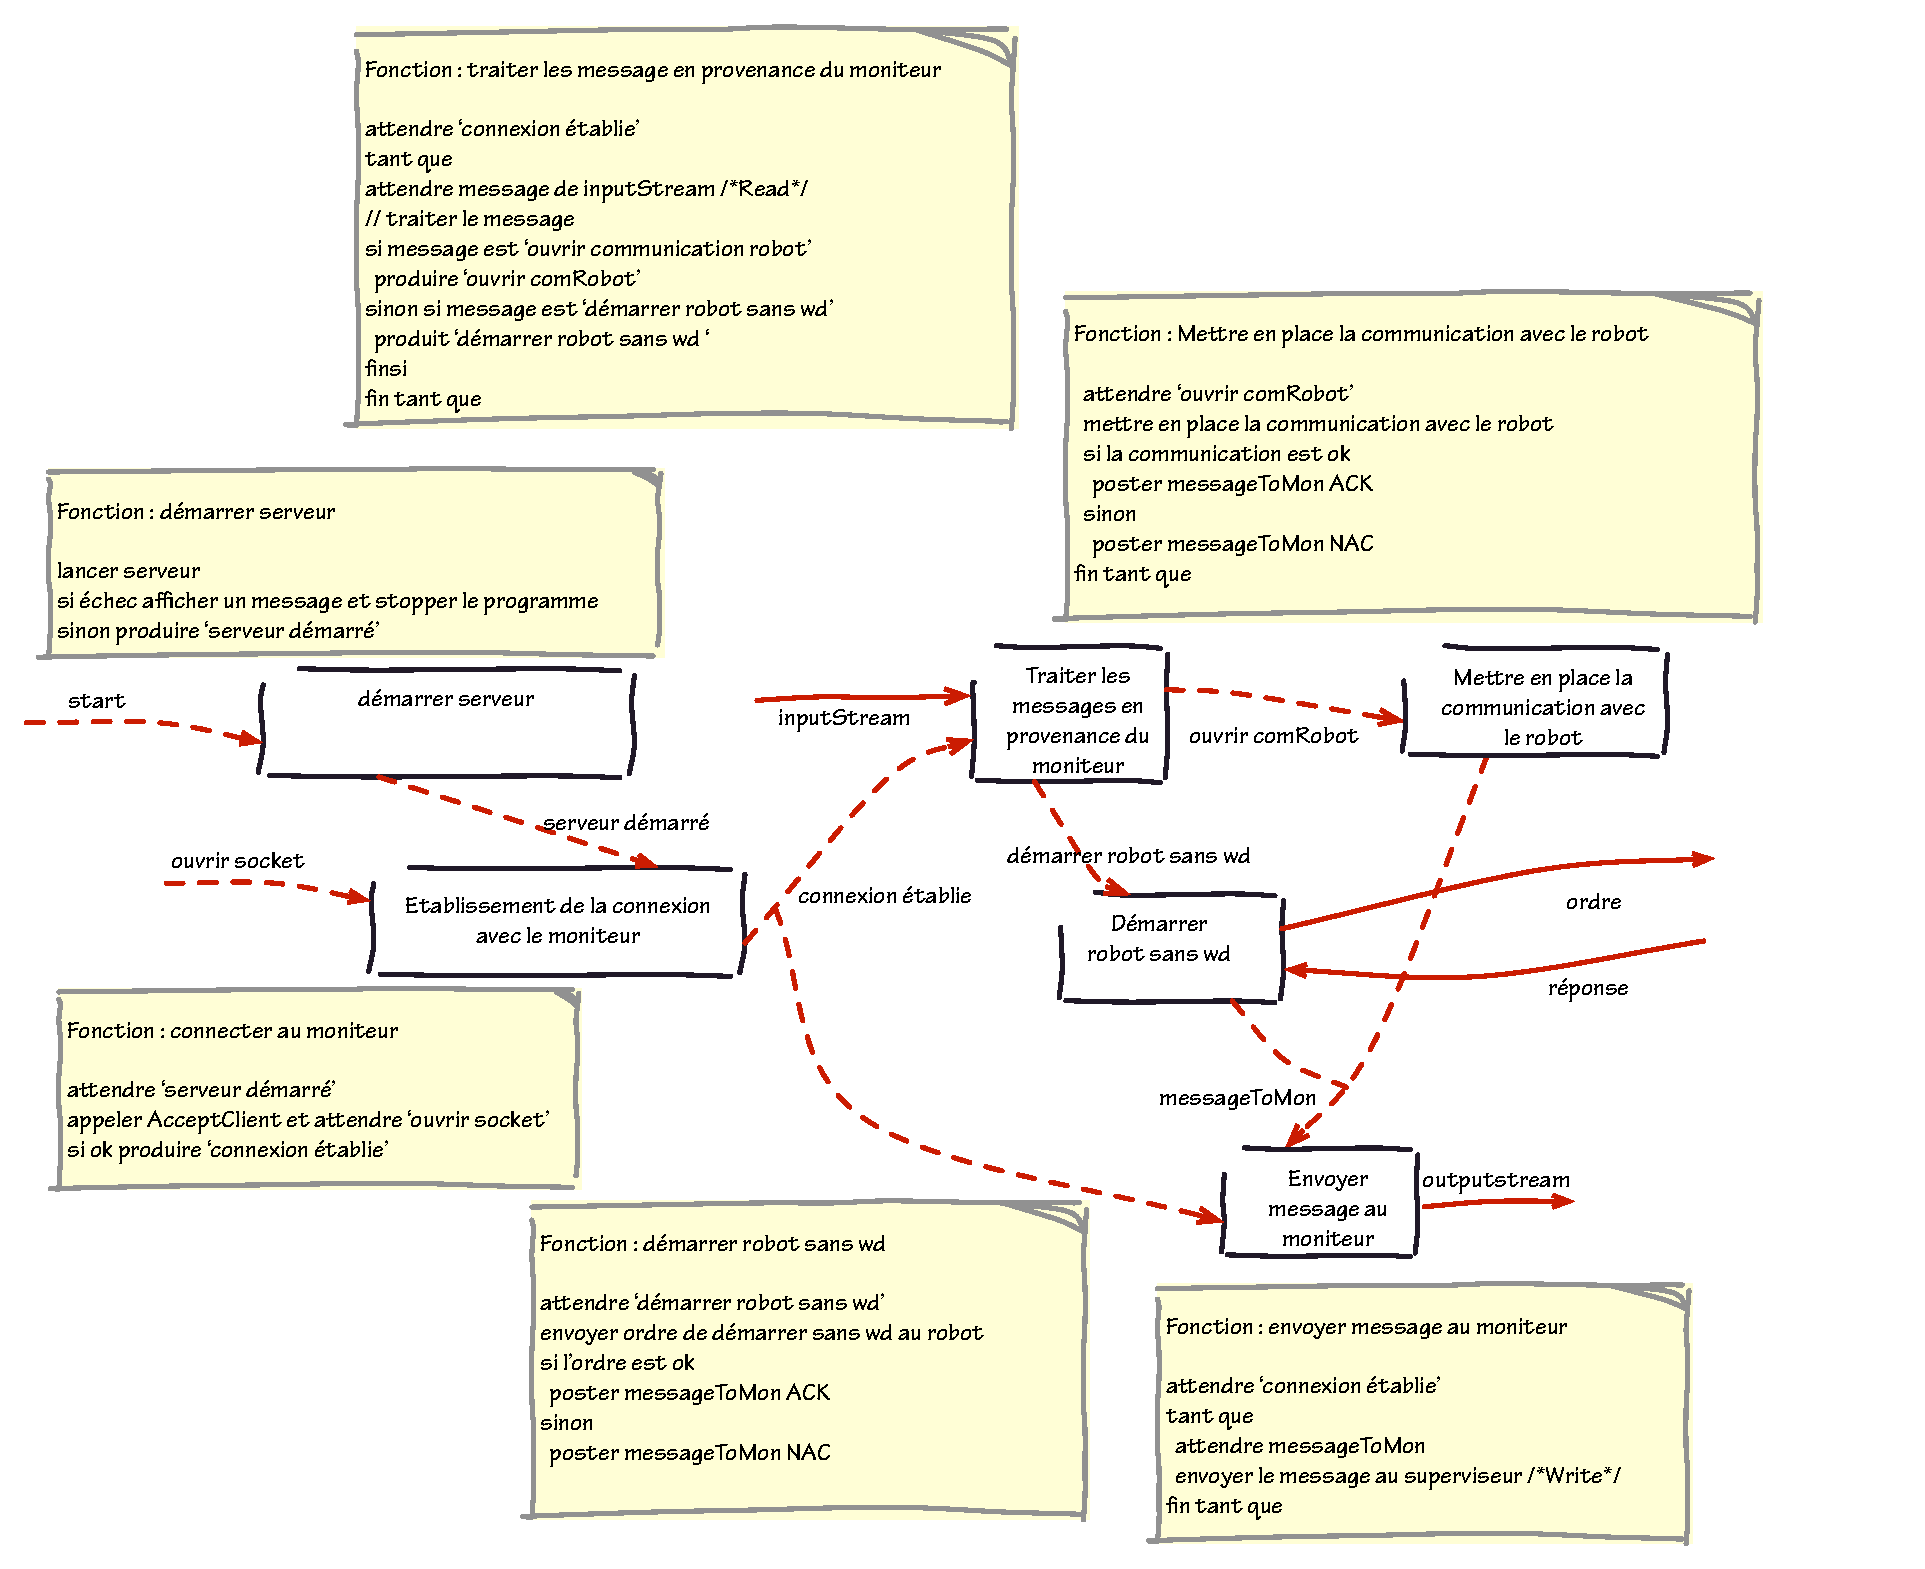
\includegraphics[scale=0.5]{figures_pdf/fonc/fonc10}
\end{center}
\end{figure}
\FloatBarrier

La dernière fonctionnalité qui sera traitée dans cette conception introduit deux variables partagées : {\tt mouvement} et {\tt robot démarré}. Le choix fait par le concepteur pour traiter les mouvements consiste à envoyer périodiquement un message de mouvement au robot. Pour cela la fonction lit le mouvement à réaliser dans la variable {\tt mouvement}. Cette variable est mise à jour lorsqu'un message de mouvement est reçu. Cependant, le message ne doit être envoyé que si le robot est démarré, d'où l'ajout de la variable {\tt robot démarré} qui est mise à jour dans la fonction qui démarre le robot.
 \begin{figure}[htbp]
\begin{center}
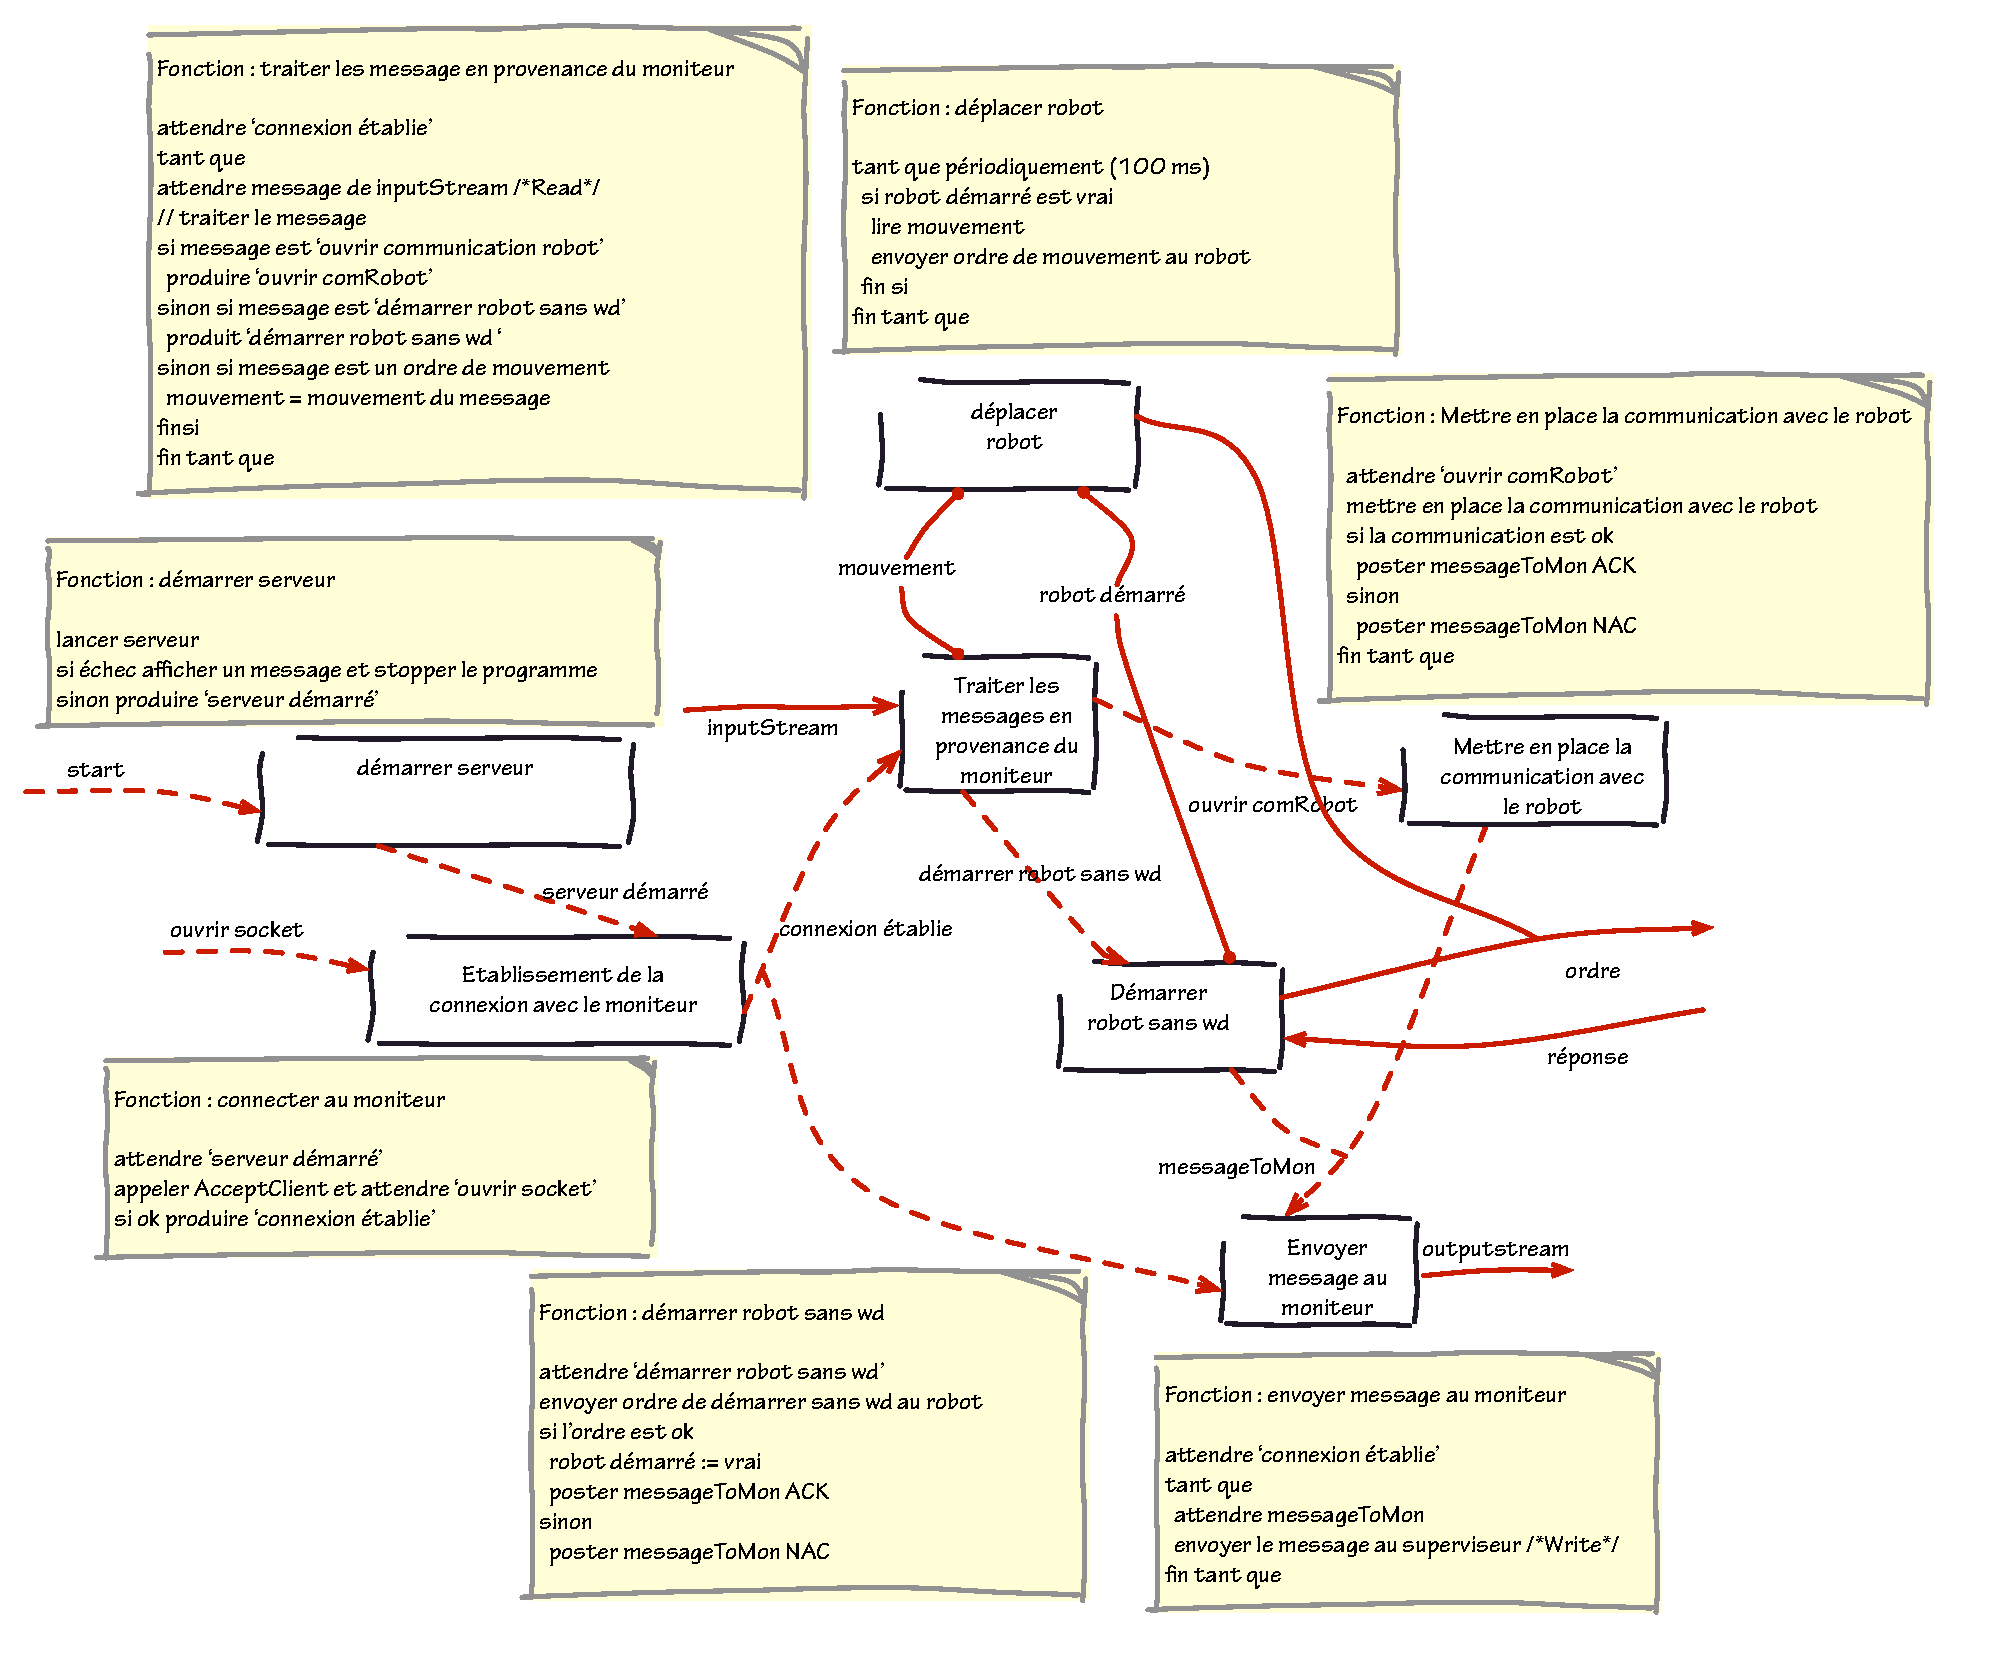
\includegraphics[scale=0.5]{figures_pdf/fonc/fonc12}
\end{center}
\end{figure}
\FloatBarrier

%%%%%%%%%%%%%%%%%%%%%%%%%
\section{Le travail d'un concepteur : la formalisation}
%%%%%%%%%%%%%%%%%%%%%%%%%

\subsection{Identification des threads}
Après avoir identifier les fonctions de l'application, le concepteur doit préciser quand l'exécution des fonctions se produit. La première étape consiste à considérer chaque fonction comme un thread. Deux questions se posent alors :
\begin{itemize}
	\item Quel est le type du thread ? Un thread apériodique (noté par un A dans un rond) est un thread dont l'exécution est contrôlé par des événements alors qu'un thread périodique (noté par la valeur de la période dans un rond) aura une exécution qui revient périodiquement.
	\item Quel est la priorité du thread ? Une règle simple pour les threads périodiques est d'attribuer les priorités par ordre décroissant des périodes, c'est-à-dire qu'un thread sera d'autant plus prioritaire que sa période sera petite.  Pour les threads apériodiques, le niveau de priorité va dépendre de la criticité des fonctions.\\
\end{itemize}

 \begin{figure}[htbp]
\begin{center}
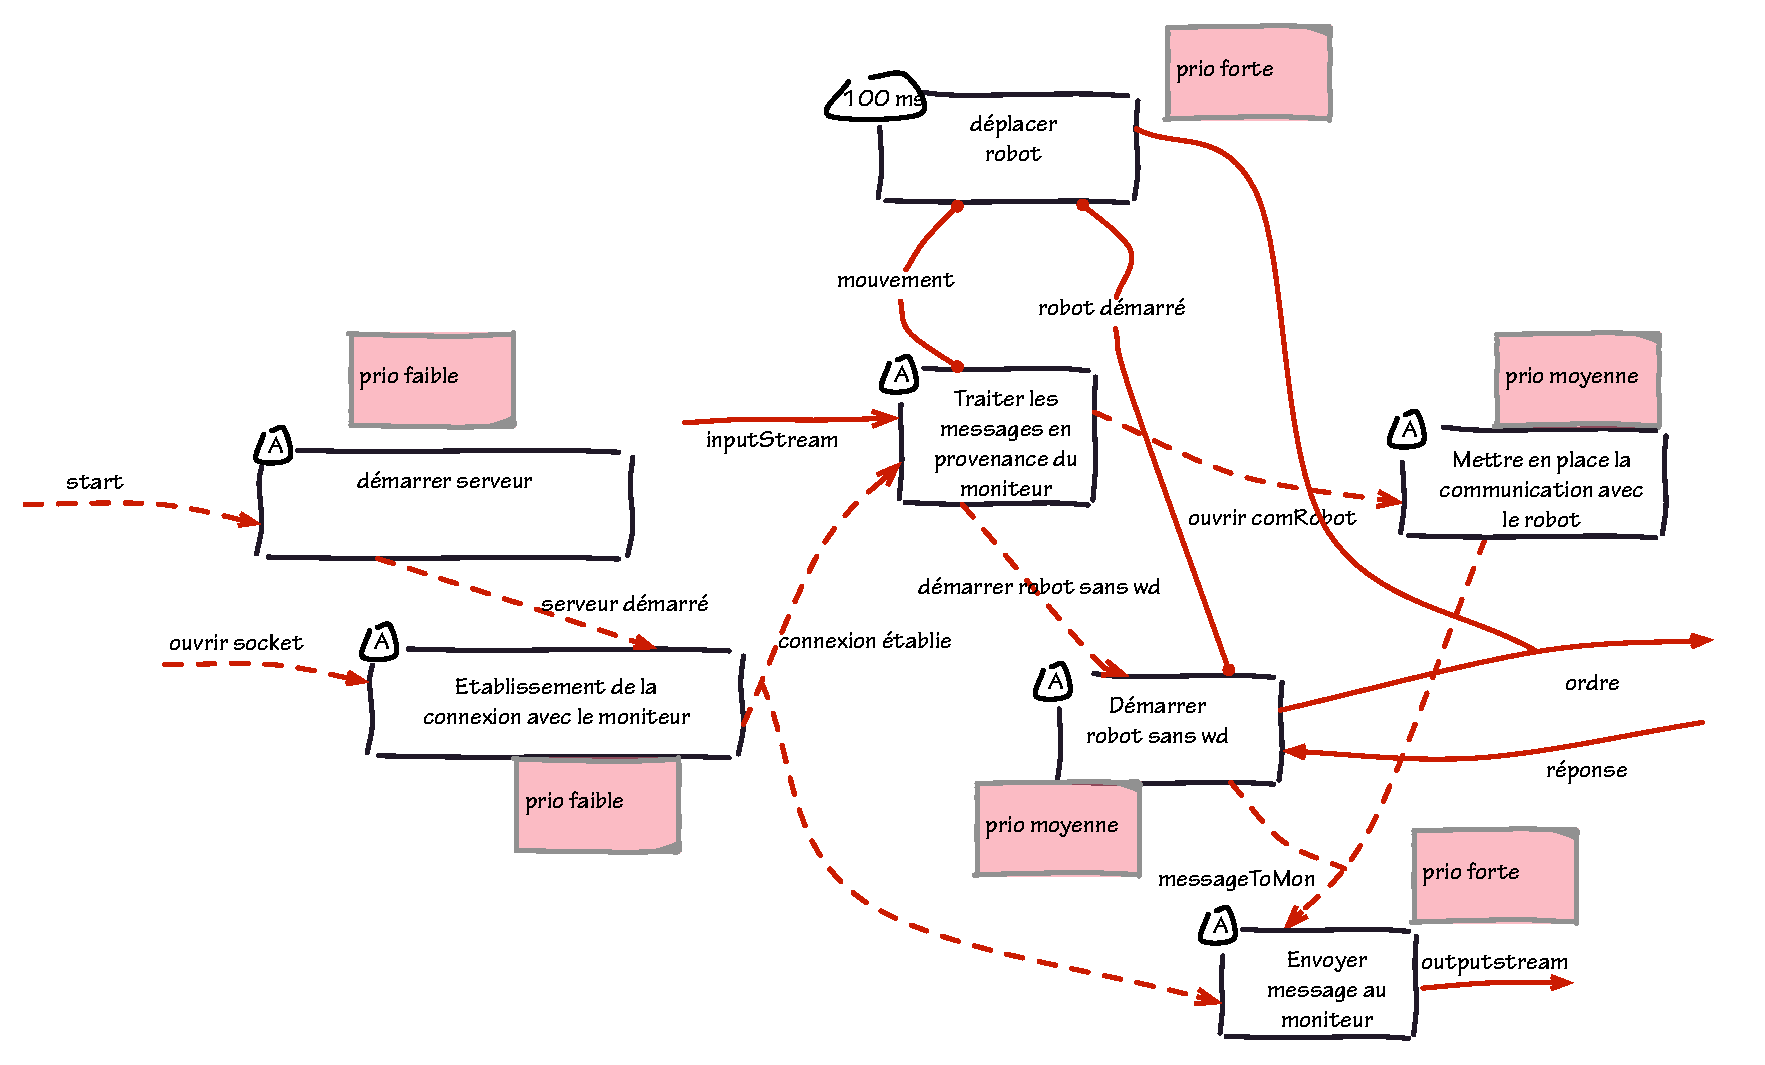
\includegraphics[scale=0.5]{figures_pdf/fonc/thread}
\end{center}
\end{figure}
\FloatBarrier

\subsection{Raffinage}

Une seconde étape consiste à avoir un regard critique sur sa conception, par exemple en se demandant s'il est possible de réunir des threads ensembles. Ici, le thread {\tt Etablissement de la communication avec le moniteur} ne peut être appelé qu'après {\tt démarrer serveur}, il est donc possible de les réunir en un seul thread.

C'est aussi le moment de se demande si toutes les fonctionnalités sont couvertes. Pour cela on reprend chaque fonctionnalité et on vérifie qu'elles sont bien traitées. Ici tout semble correct, bien qu'un doute subsiste pour la gestion des déplacements du robot...

%%%%%%%%%%%%%%%%%%%%%%%%%%%%%%%%%
\subsection{Formalisation}

Jusqu'ici tout a été réalisé au brouillon par le concepteur, il faut donc maintenant passer à une étape de formalisation pour pouvoir partager le travail réalisé et lever toute ambiguité. Pour cela, l'architecture sera décrite en AADL et le comportement des threads par des diagrammes d'activité UML. Le schéma~\ref{fig:AADL} présente le modèle AADL de l'architecture logicielle.

 \begin{figure}[htbp]
\begin{center}
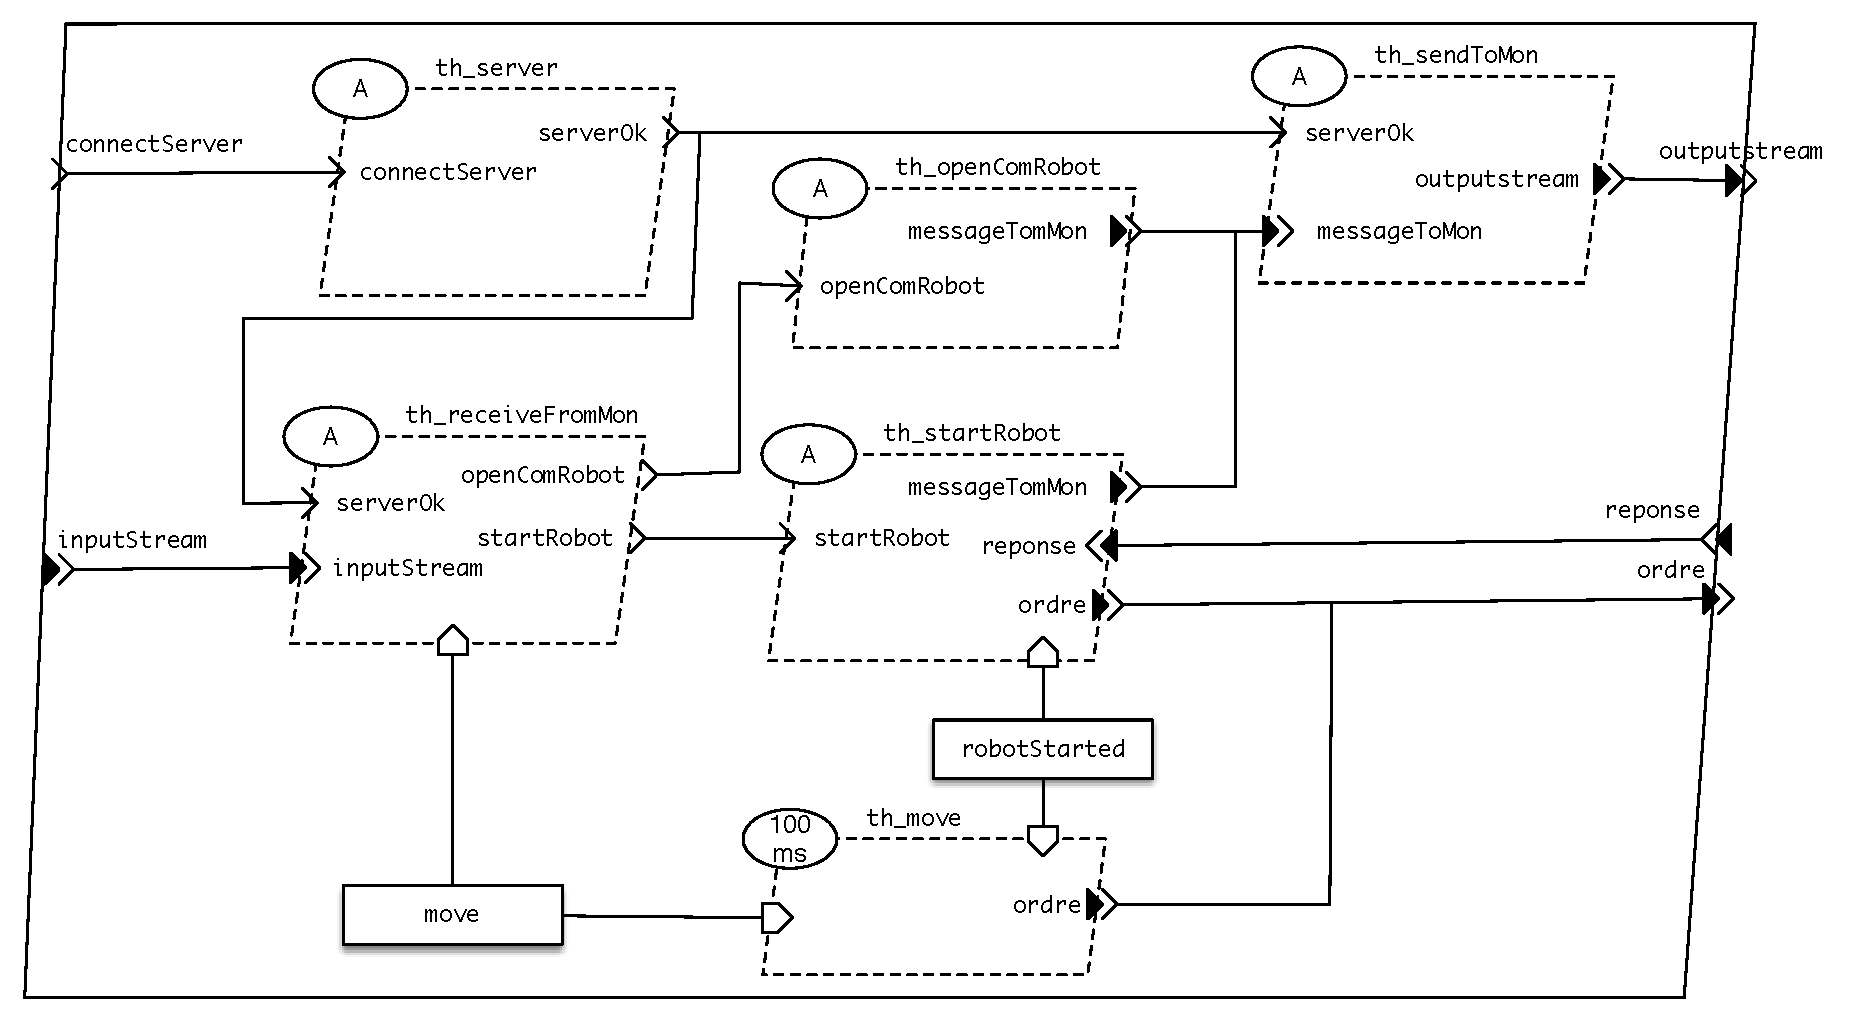
\includegraphics[scale=0.5]{figures_pdf/fonc/AADL}
\end{center}
\caption{Modèle AADL de l'architecture de l'application}
\label{fig:AADL}
\end{figure}
\FloatBarrier

Ensuite, pour chacun des threads, un diagramme d'activité UML est utilisé pour décrire son comportement. Les diagrammes ont été produits avec \href{https://www.planttext.com}{https://www.planttext.com} et les codes sources sont disponibles en annexe (disponibles numériquement sur la page moodle).

\subsection{Thread th\_server}
%@startuml
%skinparam monochrome true
%start
%:err = run_nodejs();
%if (err) then (failed)
%    :print("Failed to start nodejs");
%stop
%else (succeed)
%    :open_server();
%    :serverOk!;
%    stop
%endif
%@enduml
 \begin{figure}[htbp]
\begin{center}
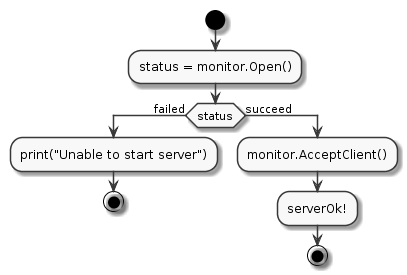
\includegraphics[scale=0.4]{figures_pdf/activity/th_server}
\end{center}
\caption{Diagramme d'activité du thread th\_server}
\end{figure}
\FloatBarrier

\subsection{Thread th\_sendToMon}
%@startuml
%skinparam monochrome true
%start
%:serverOK?;
%while ()
%  :messageToMon?header,data;
%  :send_message_to_monitor(header,data);
%endwhile
%stop
%@enduml
 \begin{figure}[htbp]
\begin{center}
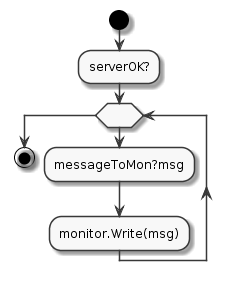
\includegraphics[scale=0.4]{figures_pdf/activity/th_sendToMon}
\end{center}
\caption{Diagramme d'activité du thread th\_sendToMon}
\end{figure}
\FloatBarrier


\subsection{Thread th\_receiveFromMon}
%@startuml
%skinparam monochrome true
%start
%:serverOk?;
%while ()
%  :receive_message_from_monitor(header,data);
%  if (header) then (HEADER_MTS_COM_DMB)
%    if (data) then (OPEN_COM_DMB)
%    :openComRobot!;
%    endif
%    else (HEADER_MTS_DMB_ORDER)
%    if (data) then (DMB_START_WITHOUT_WD)
%    :startRobot!;
%    else (DMB_GO_FORWARD || DMB_GO_BACK 
%    || DMB_GO_LEFT || DMB_GO_RIGHT 
%    || DMB_STOP_MOVE)
%    :move = data;
%    endif
%  endif
%endwhile
%stop
%@enduml
%
 \begin{figure}[htbp]
\begin{center}
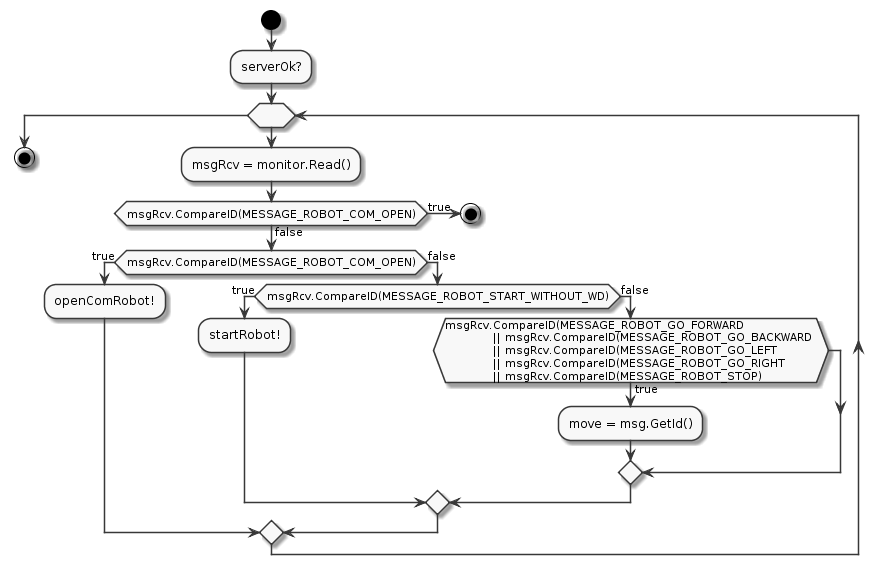
\includegraphics[scale=0.4]{figures_pdf/activity/th_receiveFromMon}
\end{center}
\caption{Diagramme d'activité du thread th\_receiveFromMon}
\end{figure}
\FloatBarrier

\subsection{Thread th\_openComRobot}
%@startuml
%skinparam monochrome true
%start
%while ()
%  :openComRobot?;
%  :err = open_communication_robot();
%  if (err) then (robot_ok)
%  :messageToMon!ACK;
%  else
%  :messageToMon!NAC;
%  endif
%endwhile
%stop
 \begin{figure}[htbp]
\begin{center}
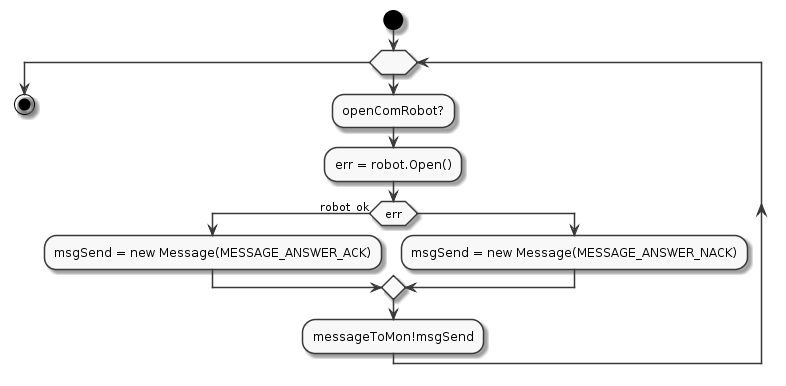
\includegraphics[scale=0.4]{figures_pdf/activity/th_openComRobot}
\end{center}
\caption{Diagramme d'activité du thread th\_openComRobot}
\end{figure}
\FloatBarrier

\subsection{Thread th\_openStartRobot}
%@startuml
%skinparam monochrome true
%start
%while ()
%  :startRobot?;
%  :err = send_command_robot(START_WITHOUT_WD);
%  if (err) then (robot_ok)
%  :messageToMon!ACK;
%  :robotStarted = true;
%  else
%  :messageToMon!NAC;
%  endif
%endwhile
%stop
%@enduml
%
 \begin{figure}[htbp]
\begin{center}
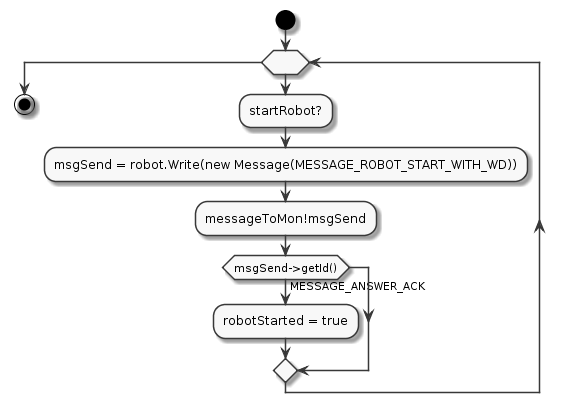
\includegraphics[scale=0.4]{figures_pdf/activity/th_startRobot}
\end{center}
\caption{Diagramme d'activité du thread th\_startRobot}
\end{figure}
\FloatBarrier

\subsection{Thread th\_move}
%@startuml
%skinparam monochrome true
%start
%:start_period(100 ms);
%while ()
%  :wait_next_period();
%  if (robotStarted) then (true)
%  :send_command_robot(move);
%  endif
%endwhile
%stop
%@enduml
 \begin{figure}[htbp]
\begin{center}
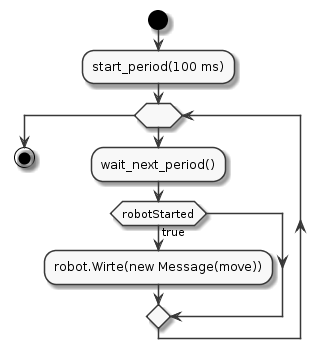
\includegraphics[scale=0.4]{figures_pdf/activity/th_move}
\end{center}
\caption{Diagramme d'activité du thread th\_move}
\end{figure}
\FloatBarrier


\newpage
%%%%%%%%%%%%%%%%%%%%%%%
\begin{appendices}
%%%%%%%%%%%%%%%%%%%%%%%%%

\section{Diagramme d'activité} 
\label{ann:diag_act}

\framebox[\textwidth]{
\begin{minipage}{0.9\textwidth}
{\bf Remarque :} Cette présentation du diagramme d'activité est tirée du \href{http://laurent-audibert.developpez.com/Cours-UML/}{cours mis en ligne} de Laurent Audibert.

Elle ne se veut pas exhaustive, mais simplement présenter les éléments nécessaire pour l'activité concernée par ce cours. De plus des éléments non standardisés sont introduit pour facilité l'expression des besoins.
\end{minipage}
}
\vspace{2mm}

Le diagramme d'activité est un diagramme comportemental d'UML, permettant de représenter le déclenchement d'événements en fonction des états du système et de modéliser des comportements parallélisables (multi-threads ou multi-processus).

Les diagrammes d'activités permettent de spécifier des traitements a priori séquentiels et offrent une vision très proche de celle des langages de programmation impératifs comme C++ ou Java. Il serait utilisé ici dans ce but.

\subsection{N{\oe}uds d'activité}

Une activité modélise un comportement décrit par un séquencement organisé d'unités dont les éléments simples sont les actions. Le flot d'exécution est modélisé par des n{\oe}uds reliés par des arcs (transitions). Le flot de contrôle reste dans l'activité jusqu'à ce que les traitements soient terminés.

Un n{\oe}ud d'activité est un type d'élément abstrait permettant de représenter les étapes le long du flot d'une activité. Il existe plusieurs familles de n{\oe}uds d'activités :
\begin{itemize}
\item les n{\oe}uds d'exécutions,
\item et les n{\oe}uds de contrôle.
\end{itemize}
La figure~\ref{fig:noeuds_act} représente les différents types de n{\oe}uds d'activité.

 \begin{figure}[htbp]
\begin{center}
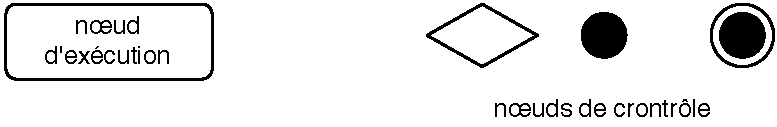
\includegraphics[scale=0.6]{figures_pdf/noeud_activite}
\caption{Représentation graphique des n{\oe}uds d'activité}
\label{fig:noeuds_act}
\end{center}
\end{figure}
\FloatBarrier

Le passage d'une activité vers une autre est matérialisé par une transition. Elles sont déclenchées dès que l'activité source est terminée et provoquent automatiquement et immédiatement le début de la prochaine activité à déclencher (l'activité cible). Contrairement aux activités, les transitions sont franchies de manière atomique, en principe sans durée perceptible.

Les transitions spécifient l'enchaînement des traitements et définissent le flot de contrôle. Elles sont représentées graphiquement par un arc entre deux n{\oe}uds. 

\subsubsection{N{\oe}uds de contrôle}
Un n{\oe}ud de contrôle est un n{\oe}ud d'activité abstrait utilisé pour coordonner les flots entre les n{\oe}uds d'une activité.
Il existe plusieurs types de n{\oe}uds de contrôle (voir figure~\ref{fig:exe_act}) :
\begin{itemize}
\item n{\oe}ud initial : Un n{\oe}ud initial est un n{\oe}ud de contrôle à partir duquel le flot débute lorsque l'activité enveloppante est invoquée. Un n{\oe}ud initial possède un arc sortant et pas d'arc entrant.
\item n{\oe}ud de fin d'activité : Lorsque l'un des arcs d'un n{\oe}ud de fin d'activité est activé (i.e. lorsqu'un flot d'exécution atteint un n{\oe}ud de fin d'activité), l'exécution de l'activité enveloppante s'achève et tout n{\oe}ud ou flot actif au sein de l'activité enveloppante est abandonné.
\item n{\oe}ud de décision : Un n{\oe}ud de décision est un n{\oe}ud de contrôle qui permet de faire un choix entre plusieurs flots sortants. Il possède un arc entrant et plusieurs arcs sortants. Ces derniers sont généralement accompagnés de conditions de garde pour conditionner le choix. L'utilisation d'une garde [else] est recommandée après un n{\oe}ud de décision car elle garantit un modèle bien formé. En effet, la condition de garde [else] est validée si et seulement si toutes les autres gardes des transitions ayant la même source sont fausses.
\item n{\oe}ud de fusion : Un n{\oe}ud de fusion est un n{\oe}ud de contrôle qui rassemble plusieurs flots alternatifs entrants en un seul flot sortant. Il n'est pas utilisé pour synchroniser des flots concurrents mais pour accepter un flot parmi plusieurs.
\end{itemize}

 \begin{figure}[htbp]
\begin{center}
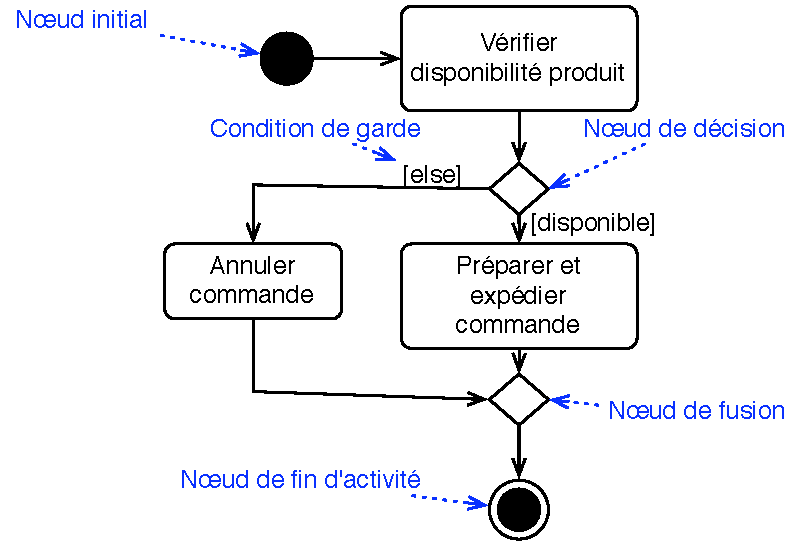
\includegraphics[scale=0.6]{figures_pdf/exe_act}
\caption{Exemple de n{\oe}uds de contrôle}
\label{fig:exe_act}
\end{center}
\end{figure}
\FloatBarrier

\subsection{N{\oe}uds d'exécution}

Un n{\oe}ud d'exécution est un n{\oe}ud d'activité exécutable qui constitue l'unité fondamentale de fonctionnalité exécutable dans une activité. L'exécution d'une action représente une transformation ou un calcul quelconque dans le système modélisé. Les actions sont généralement liées à des opérations qui sont directement invoquées. Un n{\oe}ud d'exécution doit avoir au moins un arc entrant.

Graphiquement, un n{\oe}ud d'exécution est représenté par un rectangle aux coins arrondis (figure~\ref{fig:exe_act}) qui contient sa description textuelle. Cette description textuelle peut aller d'un simple nom à une suite d'actions réalisées par l'activité. UML n'impose aucune syntaxe pour cette description textuelle, on peut donc utiliser une syntaxe proche de celle d'un langage de programmation particulier ou du pseudo-code.


\paragraph{Ajout de sémantique}
Pour faire le lien avec la conception en AADL, nous ajoutons deux actions spécifiques à la gestion des événements. Le caractère \og ? \fg utilisé après le nom d'un événement signifie que l'action est une attente (donc bloquée) sur la réception de cet événement, alors que \og ! \fg signifie sont émission. La figure~\ref{fig:exem_sync} donne un exemple où une activité est en attente (bloquée) de l'événement \texttt{toto} et produit l'événement \texttt{tata}.

Pour les événements portant une donnée nous ferons suivre le symbole de synchronisation par une liste de variables qui reçoivent les données. Par exemple, {\tt toto?var} signifie que l'action est en attente de l'événement {\tt toto} et qu'à la réception la variable {\tt var} aura pour valeur celle transmise.

 \begin{figure}[htbp]
\begin{center}
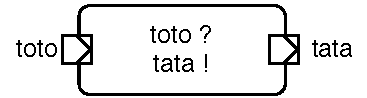
\includegraphics[scale=0.6]{figures_pdf/exem_evt}
\caption{Exemple de synchronisation}
\label{fig:exem_sync}
\end{center}
\end{figure}
\FloatBarrier

%%%%%%%%%%%%%%%%%%%%%%%%%
\newpage
\section{Le langage AADL} 
\label{ann:aadl}
 
AADL (Architecture Analysis and Design Language) est un langage de description d'architecture pour les systèmes temps réel. Il peut être indifféremment utilisé en avionique, spatial, robotique, etc. Il a été développé suite aux retours d'expérience sur l'utilisation du langage MethaH et a été standardisé sous l'autorité de le division ASD (Avionics System Division) du SAE (International Society for Automotive Engineers).

Une première version du standard AADL (SAE AS5506) a été produite en novembre 2004. Celle courante est la 2.0~\cite{AADL:2009} et date de janvier 2009. Depuis des fournitures de documents annexes et d'outils ont été proposés.

Le langage AADL étant extrêmement riche, il est impossible d'en donner ici une vue exhaustive en quelques pages.  Nous ne présentons qu'un sous-ensemble de composants pour ne se focaliser que sur les principaux. Les personnes souhaitant approfondir le sujet peuvent se référer aux notes techniques disponibles sur le site de la SAE ou bien directement accéder au standard.

Le standard~\cite{AADL:2009} est construit sur le concept de modélisation par composant. Un composant est une entité logicielle permettant de faire un calcul ou de stocker des données. Il peut représenter aussi bien une simple fonction qu'une application complète. Un composant peut être simple ou composé, il est alors dit composite. On distingue habituellement l'interface du composant qui permet de décrire les services qu'il fournit ou requière, de son implémentation qui décrit son fonctionnement interne.

AADL permet de décrire aussi bien une architecture logicielle que matérielle et de spécifier le moteur d'exécution en terme de t‚ches concurrentes, de synchronisation et d'allocation. Le standard SAE AADL offre : 
\begin{itemize}
	\item une spécification du langage avec une syntaxe textuelle ;
	\item une sémantique et une représentation graphique ;
	\item un profil UML du SAE AADL ;
	\item d'une spécification XML/XMI comme format de modèle ;
	\item et plusieurs annexes détaillant certains points : formalisation du comportement, définition des interfaces avec le C et Ada, extension au modèle d'erreur, etc.\\
\end{itemize}

\framebox[\textwidth]{
\begin{minipage}{0.9\textwidth}
{\bf Remarque :} La description du langage qui en est donnée ci-après est loin d'être exhaustive et certaines libertés ont été prises pour l'adapter aux besoins pédagogiques.

La suite du document est directement inspirée du  \href{http://www.axlog.fr/aadl/presentation\_fr.html}{guide en ligne} fourni par la société Axlog.
\end{minipage}
}

\section{Notion de composant et syntaxe}


La description d'une architecture en AADL consiste en la description de ses composants et leur composition sous forme d'une arborescence. Cette description pouvant être contenue dans des fichiers, une base de données, etc.


Chaque composant appartient à une {\bf catégorie}. Ces catégories sont prédéfinies et se décomposent en :
\begin{itemize}
	\item Catégorie matérielle avec les composants : mémoire ({\em memory}) ; périphérique ({\em device}) ; processeur ({\em processor}) ; bus ({\em bus}).
	\item Catégorie logicielle avec les composants :  donnée ({\em data}) ; sousprogramme ({\em subprogram}) ; thread ({\em thread}) ; groupe de threads ({\em thread group}) ; processus ({\em†processs}).
	\item Catégorie composite avec les composants : système ({\em system}), composant abstrait ({\em  abstract}).\\
\end{itemize}


\subsection{Types et implémentation}

Chaque composant comprend deux parties. La première, \textbf{le type}, correspond à son interface fonctionnelle, c'est-à-dire ce qui est visible pour les autres composants. La seconde, \textbf{l'implémentation}, décrit son contenu : sous-composants, propriétés, connexions, etc.

Chaque implémentation est associée à un type. ¿ chaque type est associé aucune, une ou plusieurs implémentations. La figure~\ref{fig:type_implementation} donne un exemple de deux types de composants dont le premier est associé à deux implémentations de composants (component implementations).  Textuellement, le type est introduit par le mot décrivant le type du composant, alors que l'implémentation est décrite par le type suivi du mot {\em implementation}.


\begin{figure}[htbp]
\begin{center}
\begin{minipage}[c]{.46\linewidth}
\lstset{emph={system, end, implementation, process, processor, thread, subcomponents, properties, features, reference, applies, to, connections, features, requires, data, access, System, offset, end, behavior, res, preemptable, allocation, task, policy, is, action, period, deadline, resources, tasks, in, out, event, with, not, port},emphstyle=\textbf}
\begin{lstlisting}
system type1
end type1;

system type2
end type2;

system implementation type1.impl1
end type1.impl1;

system implementation type1.impl2
end type1.impl2;
\end{lstlisting}
\end{minipage}
\caption{Exemple de description de composants}
\label{fig:type_implementation}
\end{center}
\end{figure}

L'intérêt de scinder la description d'un composant en type et implémentation est de bien séparer ces deux points de vue. Décrire le type permet à spécifier l'interface du composant, c'est-à-dire exprimer à quoi il ressemble depuis l'extérieur. Alors que l'implémentation en représente l'intérieur. Dans la pratique, la description du type et de l'implémentation peuvent être faites par des personnes différentes, chacune ayant en charge une étape dans le raffinement de la description de l'architecture, du plus haut niveau jusqu'aux moindres détails.


\subsection{Les propriétés}

Chaque composant est caractérisé par des propriétés pouvant prendre des valeurs. Les propriétés sont prédéfinies, c'est-à-dire qu'elles sont identifiées par un nom, un type et la liste des catégories de composants sur lesquelles elles s'appliquent. Par exemple les {\em threads} disposent de propriétés telles que la période, l'échéance ou la durée d'exécution (voir figure~\ref{fig:ex_prop}).

De nouvelles propriétés et de nouveaux types de propriétés peuvent être définis par l'utilisateur et associés à tout ou partie des catégories de composants. Ce mécanisme de propriétés est un point fort d'AADL en matière d'extensibilité. Gr‚ce à lui, toute notion spécifique au besoin de l'utilisateur peut être prise en compte dans sa description.

Syntaxiquement, les propriétés sont introduites par le mot {\em properties} suivi d'une liste de propriétés séparées par un point virgule. Les valeurs associées à une propriété sont spécifiées à l'aide de "=>".

\begin{figure}[htbp]
\begin{center}
\begin{minipage}[c]{.46\linewidth}
\lstset{emph={system, end, implementation, process, processor, thread, subcomponents, properties, features, reference, applies, to, connections, features, requires, data, access, System, offset, end, behavior, res, preemptable, allocation, task, policy, is, action, period, deadline, resources, tasks, in, out, event, with, not, port},emphstyle=\textbf}
\begin{lstlisting}
thread thread1
    properties
        Period => 15 ms;
        Deadline => 10 ms;
end thread1;
\end{lstlisting}
\end{minipage}
\caption{Exemple d'un {\em thred} avec des propriétés sur sa période et son échéance}
\label{fig:ex_prop}
\end{center}
\end{figure}

\subsection{Ports et connexions}

La description des flots de données et de contrôles entre composants se fait par le moyen de {\bf ports} et de {\bf connexions}. Un port est un point d'entrée et de sortie d'un composant, c'est-à-dire une interface par où transitent les données et les événements entre les composants. Une connexion permet de relier deux ports, soit les ports de deux sous-composants, soit le port d'un sous-composant avec le port du composant le contenant. Le type et le sens entre les ports connectés doivent être identiques.

La figure~\ref{fig:connexion_graph} représente graphiquement des ports avec des connexions et la figure~\ref{fig:connexion} en donne sa syntaxe. Le système contient deux {\em process}, eux-même contenant chacun un {\em thread}. Une succession de {\em ports}, représentés par les triangles, et de connexions, représentées par les lignes, établit une communication entre les deux threads.

\begin{figure}[htbp]
\begin{center}
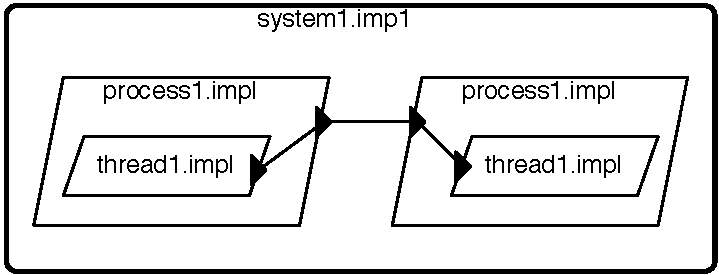
\includegraphics[scale=.6]{figures_pdf/connexion.pdf}
\caption{Représentation d'un système et de ses sous-composants}
\label{fig:connexion_graph}
\end{center}
\end{figure}

\begin{figure}[htbp]
\begin{center}
\lstset{emph={system, end, implementation, process, processor, thread, subcomponents, properties, features, reference, applies, to, connections, features, requires, data, access, System, offset, end, behavior, res, preemptable, allocation, task, policy, is, action, period, deadline, resources, tasks, in, out, event, with, not, port},emphstyle=\textbf}
\begin{minipage}[c]{.46\linewidth}
\begin{lstlisting}
system system1
end system1;

system implementation system1.impl
    subcomponents
        p1: process process1.impl;
        p2: process process2.impl;
    connections
        cn: data port p1.outport -> p2.inport;
end system1.impl;

process process1
    features
        outport: out data port;
end process1;

process implementation process1.impl
    subcomponents
        t1: thread thread1.impl;
    connections
        cn: data port t1.outport -> outport;
end process1.impl;

process process2
    features
        inport: in data port;
end process2;
\end{lstlisting}
\end{minipage}
\begin{minipage}[c]{.46\linewidth}
\begin{lstlisting}
process implementation process2.impl
    subcomponents
        t2: thread thread2.impl;
    connections
        cn: data port inport -> t2.inport;
end process2.impl;

thread thread1
    features
        outport: out data port;
end thread1;

thread implementation thread1.impl
end thread1.impl;

thread thread2
    features
        inport: in data port;
end thread2;

thread implementation thread2.impl
end thread2.impl;
\end{lstlisting}
\end{minipage}
\caption{Exemple de description de connexions}
\label{fig:connexion}
\end{center}
\end{figure}


\section{Outils}

Différentes outils existent pour manipuler le langage AADL. En particulier, l'atelier de développement ouvert TOPCASED~\cite{topcased} fournit un éditeur textuel et graphique du langage, ADELE. De même, OSATE est un outil pour vérifier la syntaxe d'une description AADL. Cependant, ces outils ne sont pas très robuste ni \og user friendly\fg.
 
\section{Description des principaux composants}

\framebox[\textwidth]{
\begin{minipage}{0.9\textwidth}
{\bf Remarque :}  Les principaux composants et éléments de description AADL utilisés pour la conception dans le cadre des TP sont énumérés dans les sections suivantes. Nous nous limitons volontairement à un sous-ensemble et ne respectons pas certaines règles imposées par le standard afin d'en simplifier son utilisation.

Nous nous limitons aussi à l'expression graphique du langage. Nous ne ferons donc pas de distinction entre type et implémentation et les propriétés seront portées sous forme d'annotations sur les composants.
\end{minipage}
}

\subsection{System}
\paragraph{Définition} Un {\em system} représente l'assemblage des composants logiciels d'une l'application et de sa plate-forme d'exécution.

\paragraph{Règles syntaxiques} Un {\em system} peut contenir les déclaration de {\em data}, de {\em port} et de {\em thread}\footnote{Cela n'est pas vrai dans le standard, un système contient normalement des {\em processes} qui contiennent des {\em threads}}.


\begin{figure}[h]
\begin{center}
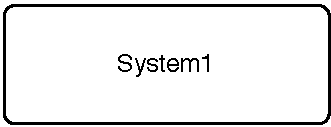
\includegraphics[scale=.6]{figures_pdf/system.pdf}
\caption{Représentation graphique d'un système}
\end{center}
\end{figure}
\FloatBarrier


%%%%%%%%%%%%%%%%%%%%
\newpage
\subsection{Thread}

\paragraph{Définition} Un {\em thread} modélise une activité concurrente, c'est-à-dire une unité ordonnançable qui peut être exécutée en concurrence avec un autre {\em thread}. Chaque {\em thread} est représenté par un flot de contrôle séquentiel qui exécute les instructions d'une image binaire produite par un code source. Un thread peut être activé ({\em dispatch}), c'est-à-dire que son exécution est provoquée par un événement qui peut être asynchrone ou périodique.

\paragraph{Règles syntaxiques} Un {\em thread} peut contenir des déclarations de {\em port}, de {\em requires data access}, et contenir des {\em data}.

\paragraph{Exécution} Un {\em thread} s'exécute à la suite d'un {\em disptach}. Un tel événement peut se produire périodiquement ou suite à un événement. Dans le cas périodique, le {\em thread} ré-exécute régulièrement le code qui lui est associé. Dans le cas d'un {\em dispatch} sur événement, le code peut faire référence à une attente de cet événement.

Quand le {\em thread} termine une exécution, il passe dans un état d'attente du prochain {\em dispatch}. Si un événement provoquant un dispatch est en attente, le {\em thread} commence immédiatement une exécution. Les événements de {\em dispatch} sur un événement peuvent être en attente.

\paragraph{Propriétés} Un {\em thread} aura une propriété décrivant son type d'activation ainsi qu'un niveau de priorité. Dans le cas périodique, une propriété indiquant la période sera ajoutée.

\begin{center}
 \begin{minipage}[c]{.46\linewidth}
 \lstset{inputencoding=utf8/latin1}
\lstset{emph={system, end, implementation, process, processor, thread, subcomponents, properties, features, reference, applies, to, connections, features, requires, data, access, System, offset, end, behavior, res, preemptable, allocation, task, policy, is, action, period, deadline, resources, tasks, in, with, not, aadlstring},emphstyle=\textbf}
%\lstset{numbers=left, numberstyle=\tiny, stepnumber=1, numbersep=10pt,numberblanklines= false} 
\begin{lstlisting}
- - Propri\'et\'es liées \`a l'activation
Dispatch_Protocol: {Periodic | Aperiodic }
Period: time
- - Propriété liée à l'ordonnancement
Priority: integer
\end{lstlisting}
\end{minipage}
\end{center}

\begin{figure}[htbp]
\begin{center}
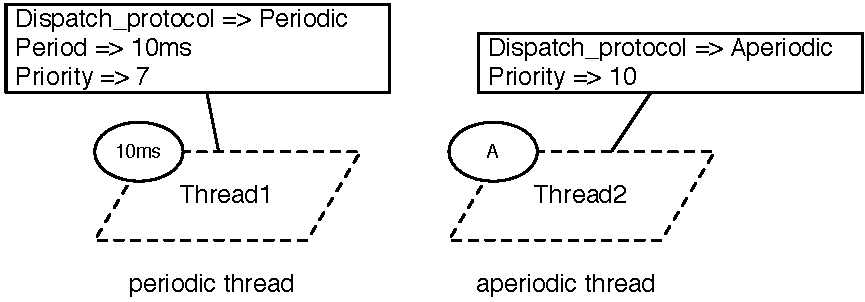
\includegraphics[scale=.6]{figures_pdf/thread.pdf}
\caption{Représentation graphique d'un {\em thread}}
\end{center}
\end{figure}
\FloatBarrier

%%%%%%%%%%%%%%%%%%%%%%%%%%%%
\subsection{Data}

\paragraph{Définition}

Un composant de type {\em data} représente une donnée qui peut être accessible et partagée par d'autres composants, ce qui est modélisé par un {\em requires data access}. L'accès concurrent à la donnée partagée est coordonnée par le protocole de partage spécifié par la propriété {\tt Concurrency\_Control\_Protocol} du composant de type {\em data}. Un  {\em thread} est considéré comme étant dans une section critique quand il a accès au composant de type {\em data}.


\paragraph{Règles syntaxiques} Un {\em data} peut contenir des déclarations de {\em subprogram access} et les propriétés associées.\\

\paragraph{Propriétés} Un {\em data} est décrit par son type ainsi que par son protocole d'accès s'il est partagé.

\begin{center}
 \begin{minipage}[c]{.8\linewidth}
  \lstset{inputencoding=utf8/latin1}
\lstset{emph={system, end, implementation, process, processor, thread, subcomponents, properties, features, reference, applies, to, connections, features, requires, data, access, System, offset, end, behavior, res, preemptable, allocation, task, policy, is, action, period, deadline, resources, tasks, in, out, event, with, not, port},emphstyle=\textbf}
\begin{lstlisting}
- - Type de la donnée
Type_Source_Name : string
- - Protocole d'accès à la donnée
Concurrency_Control_Protocol : { Maximum_Priority | Priority_Inheritance | 
                               Priority_Ceiling | Spin_Lock | Semaphore}
\end{lstlisting}
\end{minipage}
\end{center}

Un ensemble de services standards est fourni pour accéder au {\em data}. Les services {\tt Read\_Data(Data)} et {\tt Write\_Data(Data,Value)} représentent des interfaces pour les fonctions qui réalisent une lecture et écriture de la données du {\em data}. Ces fonctions commencent toujours par une prise de la ressource et se termine par sa libération. La gestion de l'accès concurrent se fait suivant le protocole spécifié. Il est bien sûr possible de définir d'autres services dédiés.


\begin{figure}[htbp]
\begin{center}
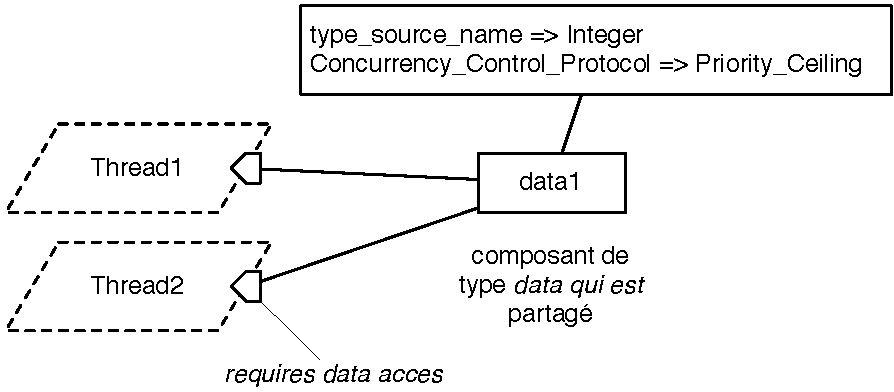
\includegraphics[scale=.6]{figures_pdf/data.pdf}
\end{center}
\end{figure}
\FloatBarrier

%%%%%%%%%%%%%
\subsection{Ports}

\paragraph{Définition} Les {\em ports} sont les points de connexion entre les différents composants qui peuvent être utilisés pour le transfère du contrôle et des données entre eux. Les {\em ports} sont directionnels, c'est-à-dire qu'un port en sortie ({\em output}) est connecté à un port en entrée ({\em input}). Les ports peuvent passés des données, des événements ou les deux. Les données transférées par les ports sont typées. Du point de vue du code source, les données des {\em ports} sont accesibles comme des variables.

Trois catégories de {\em ports} sont distinguées :
\begin{itemize}
\item Les {\em event data ports} sont les {\em ports} à travers lesquels des données sont envoyées et reçues. L'arrivée d'une donnée peut provoquer un événement chez le récepteur. Les données peuvent être mise dans une file. Un {\em event data port} représente les files de messages.
\item Les {\em data ports} sont des {\em event data ports} avec une file de taille égale à un pour laquelle seule la dernière valeure est conservée ({\em blackboard}). Par défaut, l'arrivée d'une donnée ne cause pas d'activité. Les {\em data ports} représentent les {\em ports} sans file d'attente qui communiquent des informations, tels que des flux qui sont échantillonnés.
\item Les {\em event ports} sont des {\em event data ports} sans contenu de message. Les {\em event ports} représentent des événement discrets dans l'environnement physique, tel que l'appui sur un bouton, une interruption d'horloge ou un événement logique discret comme une alarme.
\end{itemize}

Les {\em ports} sont directionnels. Un {\em out port} représente une sortie produite par un émetteur, et un {\em in port} représente une entrée requise par un récepteur.

\paragraph{Règles syntaxiques} Les {\em ports} peuvent être déclarés dans les types des {\em threads} et {\em system}.

\paragraph{Propriétés} \`A un port est associé au type de données qu'il transporte ainsi que la taille de sa file d'attente et le protocole utilisé pour gérer la file.

\begin{center}
 \begin{minipage}[c]{.72\linewidth}
 \lstset{inputencoding=utf8/latin1}
\lstset{emph={system, end, implementation, process, processor, thread, subcomponents, properties, features, reference, applies, to, connections, features, requires, data, access, System, offset, end, behavior, res, preemptable, allocation, task, policy, is, action, period, deadline, resources, tasks, in, out, event, with, not, port, enumeration, aadlstring, aadlinteger},emphstyle=\textbf}
\begin{lstlisting}
- - Taille de la file de messages, 1 par défaut
Queue_Size: aadlinteger 0 .. Max_Queue_Size => 1
\end{lstlisting}
\end{minipage}
\end{center}

Les {\em event} et {\em event data ports} ont par défaut une file associée avec une taille de 1 qui peut être explicitement changée en modifiant la propriété {\tt Queue\_size}. Les propriétés {\tt Queue\_Size} et {\tt Queue\_Processing\_Protocol} spécifient le comportement de la file.

\begin{figure}[htbp]
\begin{center}
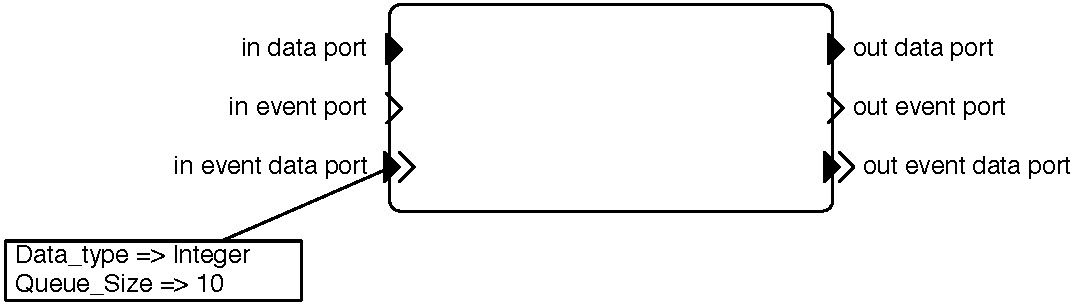
\includegraphics[scale=.6]{figures_pdf/ports.pdf}
\caption{Représentation graphique des {\em ports}}
\end{center}
\end{figure}
\FloatBarrier

%%%%%%%%%%%%%
\subsection{Connexions}

\paragraph{Définition} Une connexion est un lien orienté entre les {\em features} de deux composants qui représente les échanges de données et de contrôle entres les composants. Cela peut être la transmission de contrôle et de données entre des ports de différents {\em threads} ou entre des {\em threads} et un {\em data}.

\paragraph{Règles syntaxiques} Une connexion doit contenir au moins une source et une destination et respecter le sens de communication des {\em ports}.


\begin{figure}[htbp]
\begin{center}
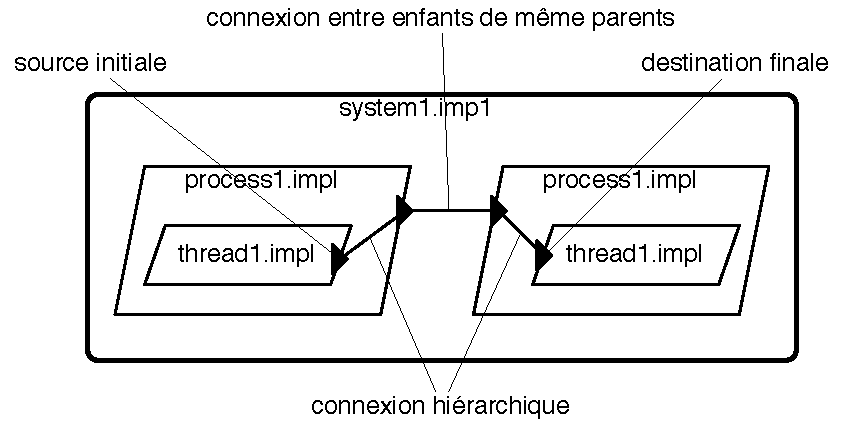
\includegraphics[scale=.6]{figures_pdf/connexion2.pdf}
\caption{Représentation graphique des connexions}
\end{center}
\end{figure}
\FloatBarrier

%%%%%%%%%%%%%
\newpage
\section{Code source des schémas d'activité}

\begin{multicols}{2}
\subsection{Thread th\_server}
{\scriptsize
\begin{verbatim}
@startuml
skinparam monochrome true
start
:monitor = new ComMonitor()
:err = monitor.Open();
if (err) then (failed)
    :print("Failed to start server");
stop
else (succeed)
    :monitor.AcceptClient();
    :serverOk!;
    stop
endif
@enduml
\end{verbatim}}

\subsection{Thread th\_sendToMon}
{\scriptsize
\begin{verbatim}
@startuml
skinparam monochrome true
start
:serverOK?;
while ()
  :messageToMon?msg;
  :monitor.Write(msg);
endwhile
stop
@enduml
\end{verbatim}
}

\subsection{Thread th\_receiveFromMon}
{\scriptsize
\begin{verbatim}
@startuml
skinparam monochrome true
start
:serverOk?;
while ()
  :msg = monitor.Read();
  if (msg.GetId()) then (MESSAGE_ROBOT_COM_OPEN)
    :openComRobot!;
  else (MESSAGE_ROBOT_GO_FORWARD || MESSAGE_ROBOT_GO_BACKWARD 
    || MESSAGE_ROBOT_GO_LEFT || MESSAGE_ROBOT_GO_RIGHT 
    || MESSAGE_ROBOT_STOP)
    :move = msg.GetId();
  endif
endwhile
stop
@enduml
\end{verbatim}
}

\subsection{Thread th\_openComRobot}
{\scriptsize
\begin{verbatim}
@startuml
skinparam monochrome true
start
while ()
  :openComRobot?;
  :err = robot.Open();
  : msg = new Message();
  if (err) then (robot_ok)
    :msg.SetId(MESSAGE_ANSWER_ACK);
    :messageToMon!msg;
  else
    :msg.SetId(MESSAGE_ANSWER_NACK);
    :messageToMon!msg;
  endif
endwhile
stop
@enduml
\end{verbatim}
}


\subsection{Thread th\_openStartRobot}
{\scriptsize
\begin{verbatim}
@startuml
skinparam monochrome true
start
while ()
  :startRobot?;
  :err = robot.Write(new Message(MESSAGE_ROBOT_START_WITH_WD));
  : msg = new Message();
  if (err) then (robot_ok)
    :msg.SetId(MESSAGE_ANSWER_ACK);
    :messageToMon!msg;
  :robotStarted = true;
  else
    :msg.SetId(MESSAGE_ANSWER_NACK);
    :messageToMon!msg;
  endif
endwhile
stop
@enduml
\end{verbatim}
}

\subsection{Thread th\_move}
{\scriptsize
\begin{verbatim}
@startuml
skinparam monochrome true
start
:start_period(100 ms);
while ()
  :wait_next_period();
  if (robotStarted) then (true)
  :robot.Wirte(new Message(move));
  endif
endwhile
stop
@enduml
\end{verbatim}
}
\end{multicols}

\end{appendices} 

\bibliographystyle{plain}
\bibliography{biblio}
 

\end{document}